% Options for packages loaded elsewhere
\PassOptionsToPackage{unicode}{hyperref}
\PassOptionsToPackage{hyphens}{url}
\PassOptionsToPackage{dvipsnames,svgnames,x11names}{xcolor}
%
\documentclass[
  letterpaper,
  DIV=11,
  numbers=noendperiod]{scrartcl}

\usepackage{amsmath,amssymb}
\usepackage{iftex}
\ifPDFTeX
  \usepackage[T1]{fontenc}
  \usepackage[utf8]{inputenc}
  \usepackage{textcomp} % provide euro and other symbols
\else % if luatex or xetex
  \usepackage{unicode-math}
  \defaultfontfeatures{Scale=MatchLowercase}
  \defaultfontfeatures[\rmfamily]{Ligatures=TeX,Scale=1}
\fi
\usepackage{lmodern}
\ifPDFTeX\else  
    % xetex/luatex font selection
\fi
% Use upquote if available, for straight quotes in verbatim environments
\IfFileExists{upquote.sty}{\usepackage{upquote}}{}
\IfFileExists{microtype.sty}{% use microtype if available
  \usepackage[]{microtype}
  \UseMicrotypeSet[protrusion]{basicmath} % disable protrusion for tt fonts
}{}
\makeatletter
\@ifundefined{KOMAClassName}{% if non-KOMA class
  \IfFileExists{parskip.sty}{%
    \usepackage{parskip}
  }{% else
    \setlength{\parindent}{0pt}
    \setlength{\parskip}{6pt plus 2pt minus 1pt}}
}{% if KOMA class
  \KOMAoptions{parskip=half}}
\makeatother
\usepackage{xcolor}
\setlength{\emergencystretch}{3em} % prevent overfull lines
\setcounter{secnumdepth}{-\maxdimen} % remove section numbering
% Make \paragraph and \subparagraph free-standing
\ifx\paragraph\undefined\else
  \let\oldparagraph\paragraph
  \renewcommand{\paragraph}[1]{\oldparagraph{#1}\mbox{}}
\fi
\ifx\subparagraph\undefined\else
  \let\oldsubparagraph\subparagraph
  \renewcommand{\subparagraph}[1]{\oldsubparagraph{#1}\mbox{}}
\fi

\usepackage{color}
\usepackage{fancyvrb}
\newcommand{\VerbBar}{|}
\newcommand{\VERB}{\Verb[commandchars=\\\{\}]}
\DefineVerbatimEnvironment{Highlighting}{Verbatim}{commandchars=\\\{\}}
% Add ',fontsize=\small' for more characters per line
\usepackage{framed}
\definecolor{shadecolor}{RGB}{241,243,245}
\newenvironment{Shaded}{\begin{snugshade}}{\end{snugshade}}
\newcommand{\AlertTok}[1]{\textcolor[rgb]{0.68,0.00,0.00}{#1}}
\newcommand{\AnnotationTok}[1]{\textcolor[rgb]{0.37,0.37,0.37}{#1}}
\newcommand{\AttributeTok}[1]{\textcolor[rgb]{0.40,0.45,0.13}{#1}}
\newcommand{\BaseNTok}[1]{\textcolor[rgb]{0.68,0.00,0.00}{#1}}
\newcommand{\BuiltInTok}[1]{\textcolor[rgb]{0.00,0.23,0.31}{#1}}
\newcommand{\CharTok}[1]{\textcolor[rgb]{0.13,0.47,0.30}{#1}}
\newcommand{\CommentTok}[1]{\textcolor[rgb]{0.37,0.37,0.37}{#1}}
\newcommand{\CommentVarTok}[1]{\textcolor[rgb]{0.37,0.37,0.37}{\textit{#1}}}
\newcommand{\ConstantTok}[1]{\textcolor[rgb]{0.56,0.35,0.01}{#1}}
\newcommand{\ControlFlowTok}[1]{\textcolor[rgb]{0.00,0.23,0.31}{#1}}
\newcommand{\DataTypeTok}[1]{\textcolor[rgb]{0.68,0.00,0.00}{#1}}
\newcommand{\DecValTok}[1]{\textcolor[rgb]{0.68,0.00,0.00}{#1}}
\newcommand{\DocumentationTok}[1]{\textcolor[rgb]{0.37,0.37,0.37}{\textit{#1}}}
\newcommand{\ErrorTok}[1]{\textcolor[rgb]{0.68,0.00,0.00}{#1}}
\newcommand{\ExtensionTok}[1]{\textcolor[rgb]{0.00,0.23,0.31}{#1}}
\newcommand{\FloatTok}[1]{\textcolor[rgb]{0.68,0.00,0.00}{#1}}
\newcommand{\FunctionTok}[1]{\textcolor[rgb]{0.28,0.35,0.67}{#1}}
\newcommand{\ImportTok}[1]{\textcolor[rgb]{0.00,0.46,0.62}{#1}}
\newcommand{\InformationTok}[1]{\textcolor[rgb]{0.37,0.37,0.37}{#1}}
\newcommand{\KeywordTok}[1]{\textcolor[rgb]{0.00,0.23,0.31}{#1}}
\newcommand{\NormalTok}[1]{\textcolor[rgb]{0.00,0.23,0.31}{#1}}
\newcommand{\OperatorTok}[1]{\textcolor[rgb]{0.37,0.37,0.37}{#1}}
\newcommand{\OtherTok}[1]{\textcolor[rgb]{0.00,0.23,0.31}{#1}}
\newcommand{\PreprocessorTok}[1]{\textcolor[rgb]{0.68,0.00,0.00}{#1}}
\newcommand{\RegionMarkerTok}[1]{\textcolor[rgb]{0.00,0.23,0.31}{#1}}
\newcommand{\SpecialCharTok}[1]{\textcolor[rgb]{0.37,0.37,0.37}{#1}}
\newcommand{\SpecialStringTok}[1]{\textcolor[rgb]{0.13,0.47,0.30}{#1}}
\newcommand{\StringTok}[1]{\textcolor[rgb]{0.13,0.47,0.30}{#1}}
\newcommand{\VariableTok}[1]{\textcolor[rgb]{0.07,0.07,0.07}{#1}}
\newcommand{\VerbatimStringTok}[1]{\textcolor[rgb]{0.13,0.47,0.30}{#1}}
\newcommand{\WarningTok}[1]{\textcolor[rgb]{0.37,0.37,0.37}{\textit{#1}}}

\providecommand{\tightlist}{%
  \setlength{\itemsep}{0pt}\setlength{\parskip}{0pt}}\usepackage{longtable,booktabs,array}
\usepackage{calc} % for calculating minipage widths
% Correct order of tables after \paragraph or \subparagraph
\usepackage{etoolbox}
\makeatletter
\patchcmd\longtable{\par}{\if@noskipsec\mbox{}\fi\par}{}{}
\makeatother
% Allow footnotes in longtable head/foot
\IfFileExists{footnotehyper.sty}{\usepackage{footnotehyper}}{\usepackage{footnote}}
\makesavenoteenv{longtable}
\usepackage{graphicx}
\makeatletter
\def\maxwidth{\ifdim\Gin@nat@width>\linewidth\linewidth\else\Gin@nat@width\fi}
\def\maxheight{\ifdim\Gin@nat@height>\textheight\textheight\else\Gin@nat@height\fi}
\makeatother
% Scale images if necessary, so that they will not overflow the page
% margins by default, and it is still possible to overwrite the defaults
% using explicit options in \includegraphics[width, height, ...]{}
\setkeys{Gin}{width=\maxwidth,height=\maxheight,keepaspectratio}
% Set default figure placement to htbp
\makeatletter
\def\fps@figure{htbp}
\makeatother

\KOMAoption{captions}{tableheading}
\makeatletter
\makeatother
\makeatletter
\makeatother
\makeatletter
\@ifpackageloaded{caption}{}{\usepackage{caption}}
\AtBeginDocument{%
\ifdefined\contentsname
  \renewcommand*\contentsname{Table of contents}
\else
  \newcommand\contentsname{Table of contents}
\fi
\ifdefined\listfigurename
  \renewcommand*\listfigurename{List of Figures}
\else
  \newcommand\listfigurename{List of Figures}
\fi
\ifdefined\listtablename
  \renewcommand*\listtablename{List of Tables}
\else
  \newcommand\listtablename{List of Tables}
\fi
\ifdefined\figurename
  \renewcommand*\figurename{Figure}
\else
  \newcommand\figurename{Figure}
\fi
\ifdefined\tablename
  \renewcommand*\tablename{Table}
\else
  \newcommand\tablename{Table}
\fi
}
\@ifpackageloaded{float}{}{\usepackage{float}}
\floatstyle{ruled}
\@ifundefined{c@chapter}{\newfloat{codelisting}{h}{lop}}{\newfloat{codelisting}{h}{lop}[chapter]}
\floatname{codelisting}{Listing}
\newcommand*\listoflistings{\listof{codelisting}{List of Listings}}
\makeatother
\makeatletter
\@ifpackageloaded{caption}{}{\usepackage{caption}}
\@ifpackageloaded{subcaption}{}{\usepackage{subcaption}}
\makeatother
\makeatletter
\@ifpackageloaded{tcolorbox}{}{\usepackage[skins,breakable]{tcolorbox}}
\makeatother
\makeatletter
\@ifundefined{shadecolor}{\definecolor{shadecolor}{rgb}{.97, .97, .97}}
\makeatother
\makeatletter
\makeatother
\makeatletter
\makeatother
\ifLuaTeX
  \usepackage{selnolig}  % disable illegal ligatures
\fi
\IfFileExists{bookmark.sty}{\usepackage{bookmark}}{\usepackage{hyperref}}
\IfFileExists{xurl.sty}{\usepackage{xurl}}{} % add URL line breaks if available
\urlstyle{same} % disable monospaced font for URLs
\hypersetup{
  pdftitle={Social Network Activation: Application in Smartphone Use},
  colorlinks=true,
  linkcolor={blue},
  filecolor={Maroon},
  citecolor={Blue},
  urlcolor={Blue},
  pdfcreator={LaTeX via pandoc}}

\title{Social Network Activation: \The Application in Smartphone Use}
\author{}
\date{2023-11-28}

\begin{document}
\maketitle
\ifdefined\Shaded\renewenvironment{Shaded}{\begin{tcolorbox}[interior hidden, enhanced, sharp corners, borderline west={3pt}{0pt}{shadecolor}, breakable, boxrule=0pt, frame hidden]}{\end{tcolorbox}}\fi

\hypertarget{social-network-activation}{%
\subsection{Social Network Activation}\label{social-network-activation}}

\begin{figure}

{\centering 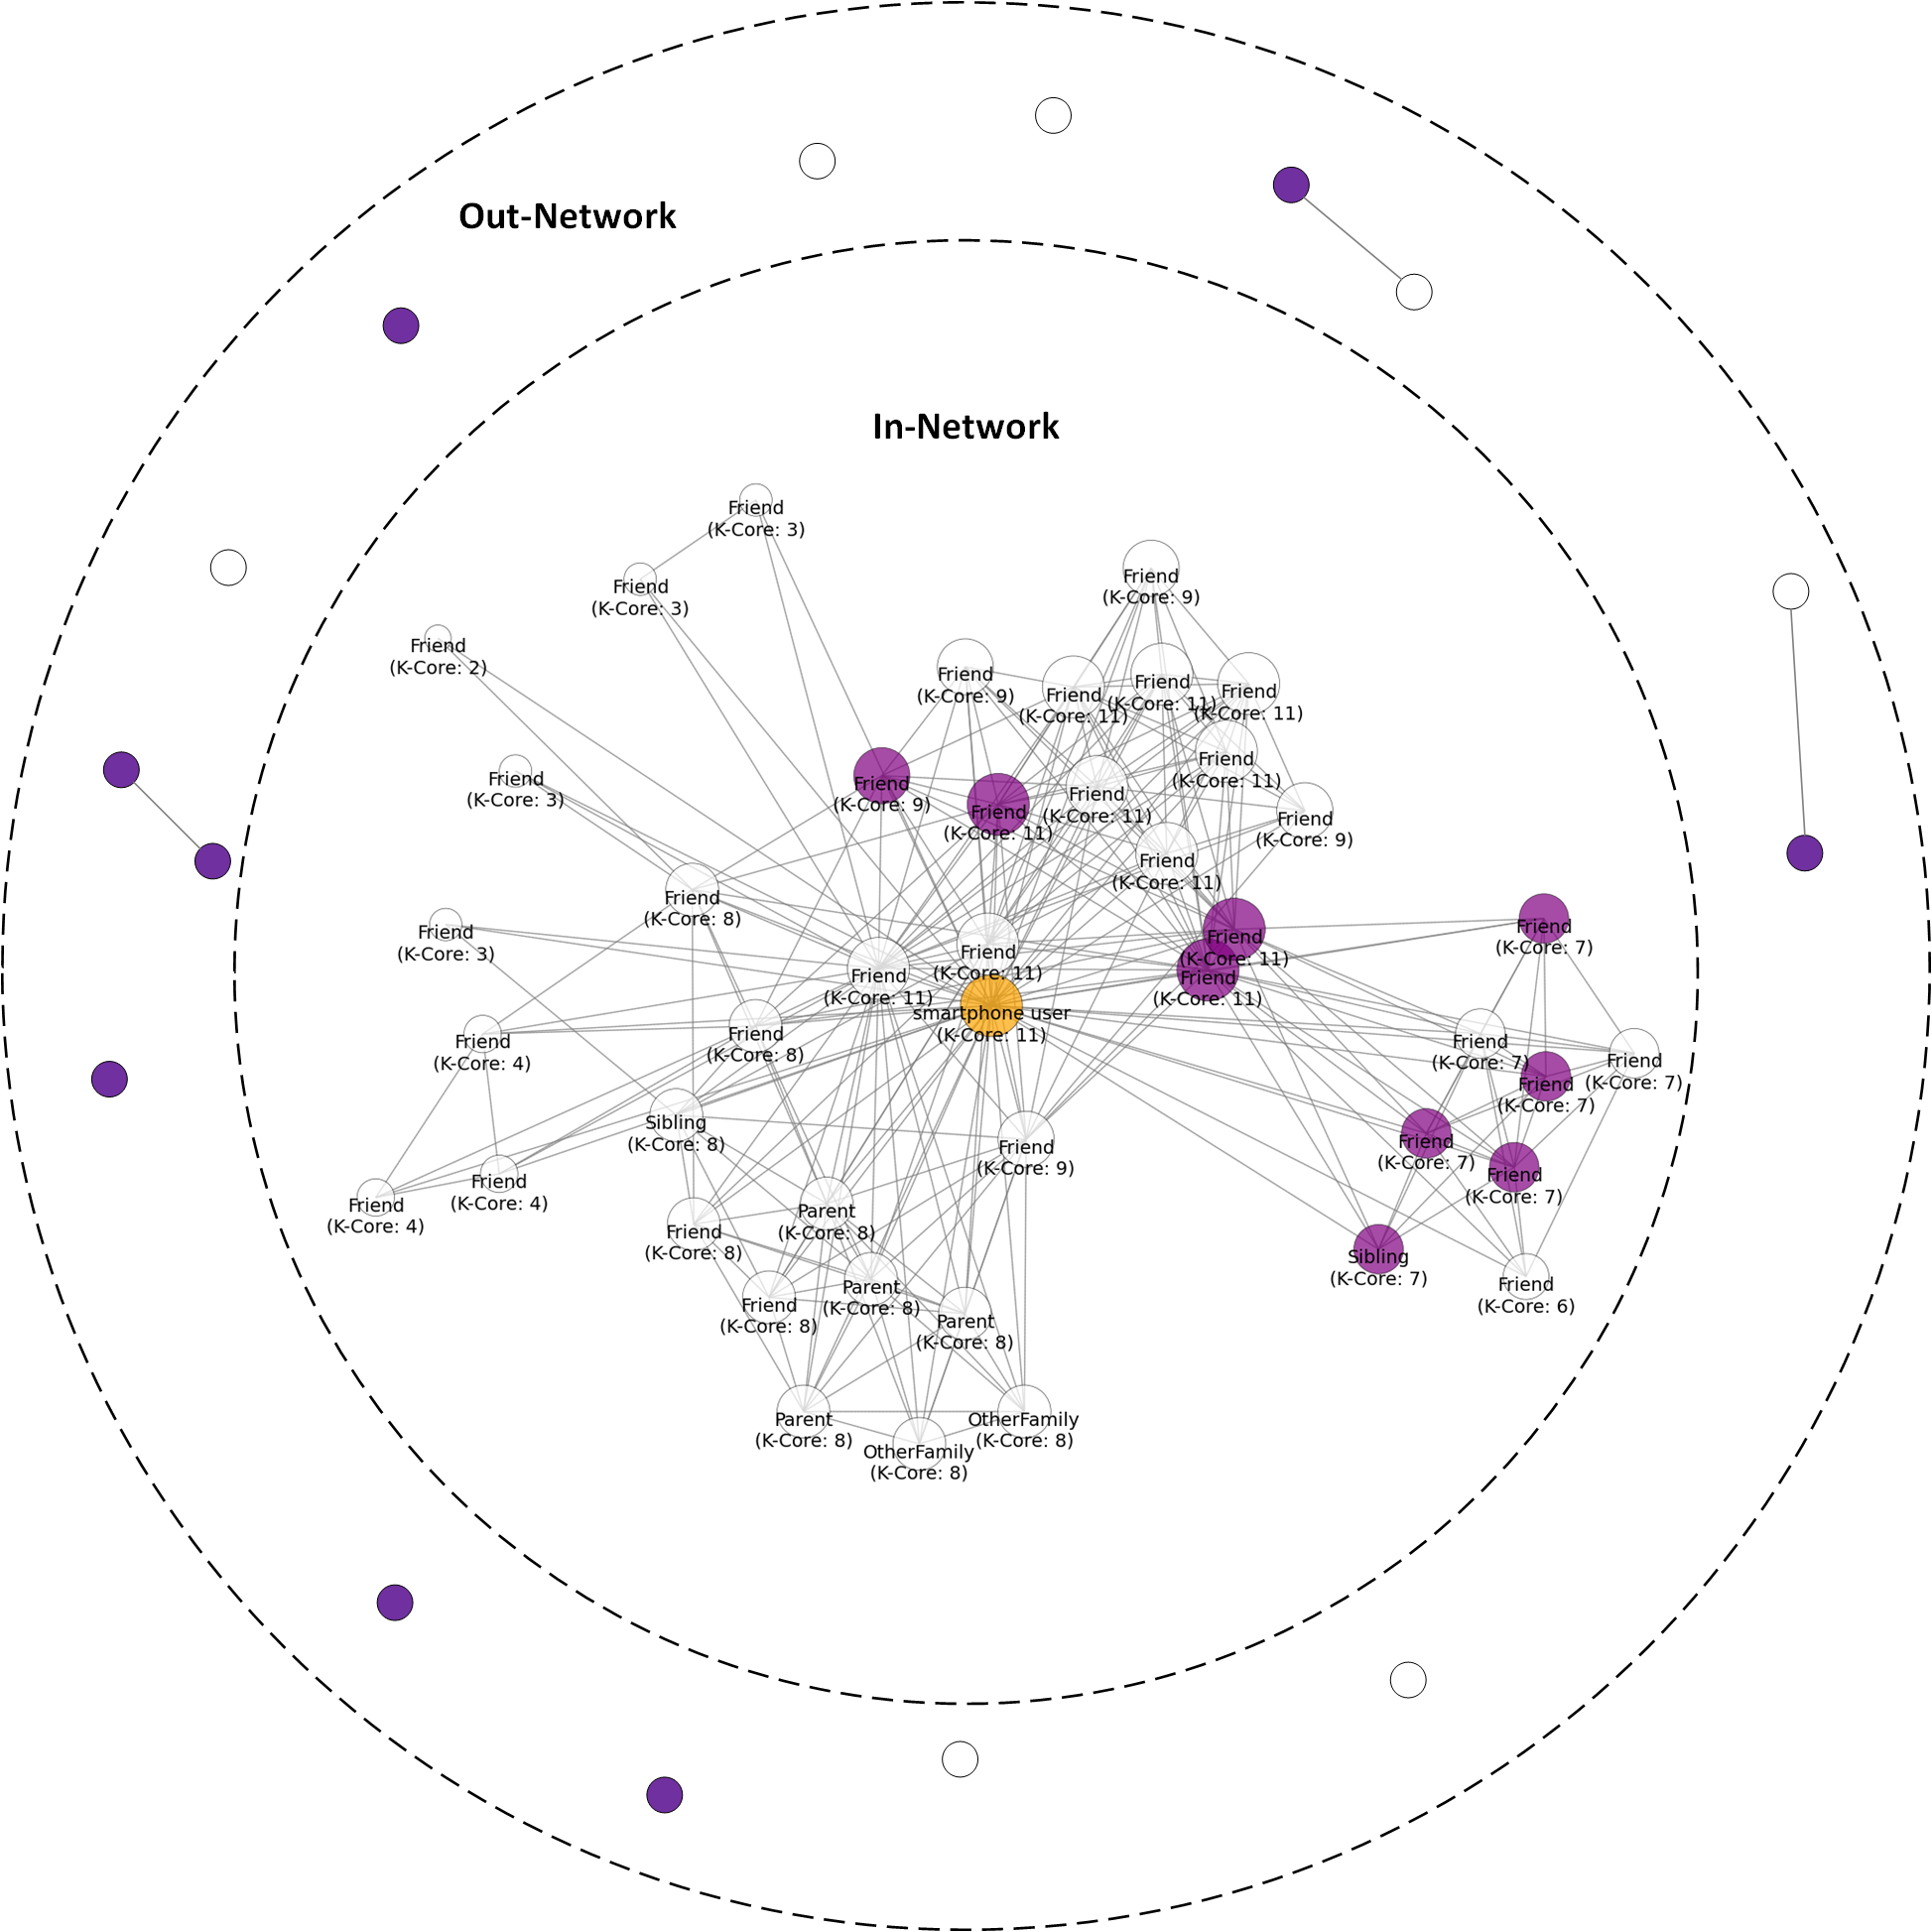
\includegraphics{inout.png}

}

\end{figure}

\hypertarget{hypothesis-1}{%
\subsection{Hypothesis 1}\label{hypothesis-1}}

\begin{figure}

{\centering 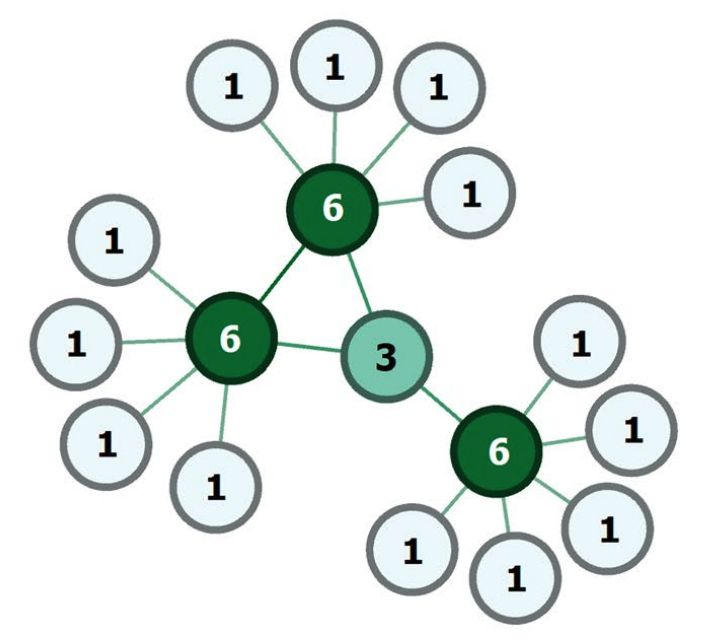
\includegraphics{images/centrality-01.png}

}

\end{figure}

\begin{itemize}
\tightlist
\item
  H1: Activating social networks with a higher \textbf{Degree
  Centrality} score \textbf{reduces} the time spent on a smartphone.
\end{itemize}

\hypertarget{hypothesis-2}{%
\subsection{Hypothesis 2}\label{hypothesis-2}}

\begin{figure}

{\centering 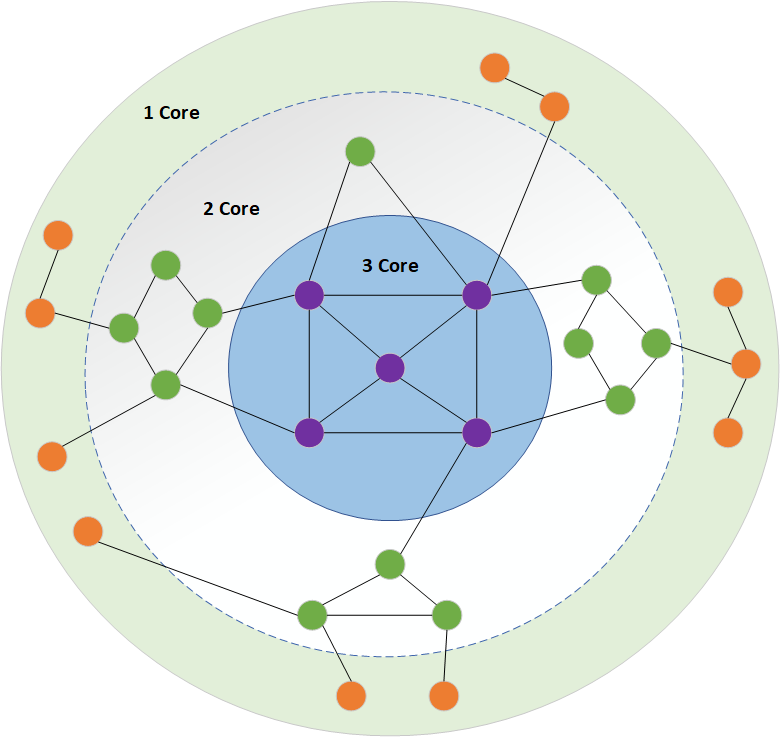
\includegraphics{images/core_number.png}

}

\end{figure}

\begin{itemize}
\tightlist
\item
  H2: Activating social networks with a higher \textbf{K-Core} score
  \textbf{reduces} the time spent on a smartphone.
\end{itemize}

\hypertarget{hypothesis-3}{%
\subsection{Hypothesis 3}\label{hypothesis-3}}

\begin{itemize}
\tightlist
\item
  H3 (1): An \textbf{increase in communication} with contacts with high
  degree centrality \textbf{improves the effectiveness} of degree
  centrality in reducing smartphone usage.
\item
  H3 (2): An \textbf{increase in communication} with contacts with high
  K-Core \textbf{improves the effectiveness} of K-Core in reducing
  smartphone usage.
\end{itemize}

\hypertarget{specification-1}{%
\subsection{Specification 1}\label{specification-1}}

\hfill\break

\(\begin{equation} \begin{split} \text{Screen Time}_{it} = \beta_0 + \beta_1 \cdot \text{Social Network Features}_{it} + \\ \alpha \cdot X_{it} + \theta_i + \lambda_t + \varepsilon_{it} \end{split} \label{e1}\end{equation}\)\\

\begin{itemize}
\tightlist
\item
  \(\text{Screen Time}_{it}\): Smartphone use time before users fall
  asleep
\item
  \(\text{Social Network Features}_{it}\): Degree Centrality and K-Core
\item
  \(\text{X}_{it}\): Control variables: Steps, sleep duration, naps,
  etc.
\item
  \(\theta_i\): Individual fixed effect (students)
\item
  \(\lambda_t\): Time fixed effect (day)
\end{itemize}

\hypertarget{result-1-main-centrality-k-core}{%
\subsection{Result 1: Main (Centrality \&
K-Core)}\label{result-1-main-centrality-k-core}}

\begin{figure}

{\centering 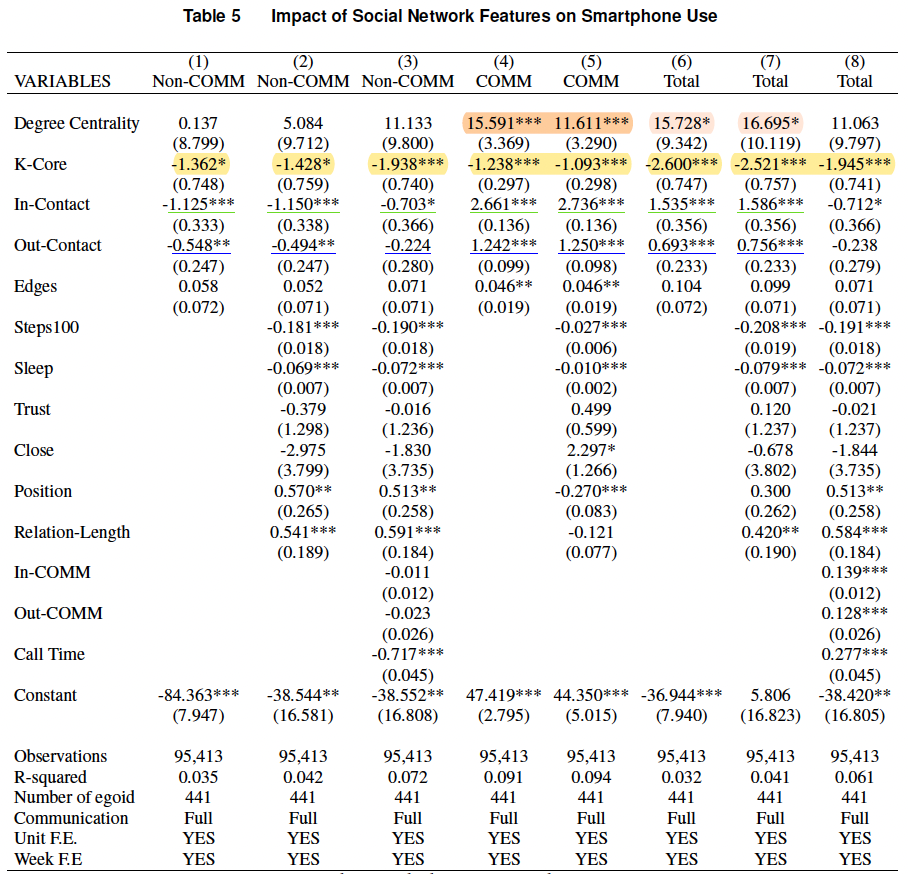
\includegraphics{images/2table5.png}

}

\end{figure}

\hypertarget{conclusion-h1-h2}{%
\subsection{Conclusion (H1 \& H2)}\label{conclusion-h1-h2}}

~

\begin{itemize}
\tightlist
\item
  Degree Centrality \textbf{does not} affect non-communication
  smartphone use but \textbf{improve}s overall smartphone use by
  increasing the time spent on communication.~\textbf{H1 is not
  supported.}
\item
  K-Core \textbf{reduces} overall smartphone use( Communication, others
  and overall). ~\textbf{H2 is supported.}
\end{itemize}

\hypertarget{result-3-moderating-impact-of-communication}{%
\subsection{Result 3: Moderating Impact of
Communication}\label{result-3-moderating-impact-of-communication}}

\begin{figure}

{\centering 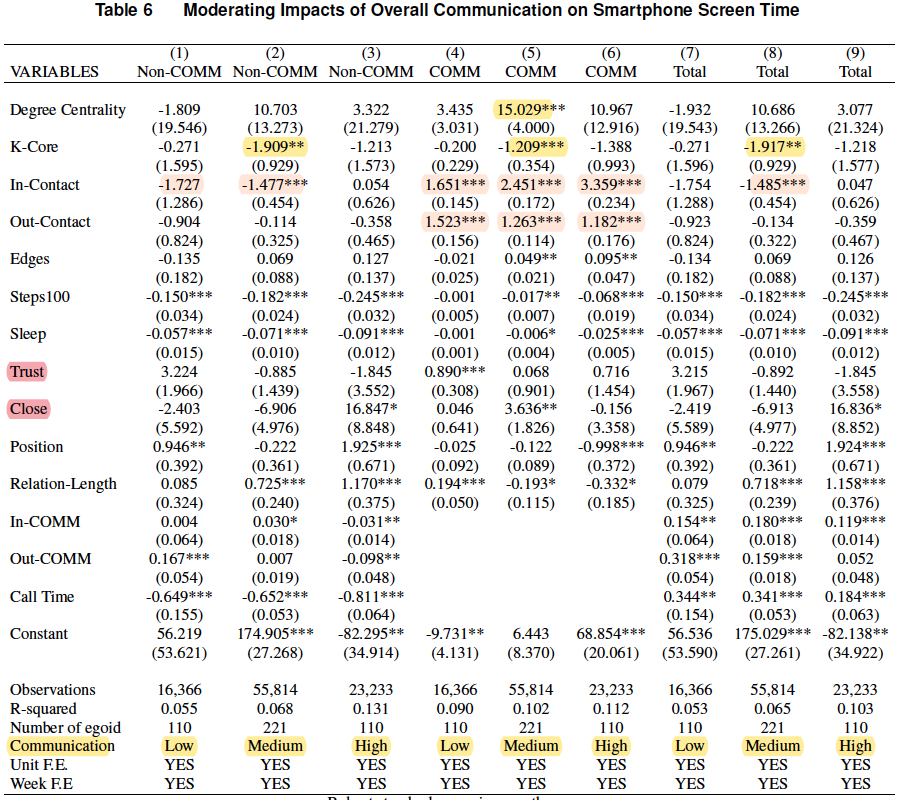
\includegraphics{images/2table6.png}

}

\end{figure}

\hypertarget{conclusion-3-h3}{%
\subsection{Conclusion 3 (H3)}\label{conclusion-3-h3}}

~

\begin{itemize}
\tightlist
\item
  Communication frequency shows \textbf{NO moderating impact} on the
  effectiveness of network features. ~\textbf{H3 is not supported.}
\end{itemize}

\hypertarget{result-4-addiction-esimation-logistic}{%
\subsection{Result 4: Addiction Esimation
(Logistic)}\label{result-4-addiction-esimation-logistic}}

\hfill\break
Addiction is defined as:

\begin{itemize}
\item
  \textbf{Overall} addiction: overall screen time \textgreater{} 300 min
\item
  \textbf{Non-communication-drive} addiction: Non-communication screen
  time \textgreater{} 240 min
\item
  \textbf{Communication-drive} addiction: Communication screen time
  \textgreater{} 40 min
\end{itemize}

\hypertarget{specification-2}{%
\subsection{Specification 2}\label{specification-2}}

~

\(\begin{equation} \begin{split} \ln \left(\frac{\operatorname{Pr}\left(\text { Addiction }_{it}=1 \mid \boldsymbol{X}_{i t}\right)}{1-\operatorname{Pr}\left(\text { Addiction }_{it}=1 \mid \boldsymbol{X}_{i t}\right)}\right) = \beta_{0}+\beta_{1} \cdot \text{Social Network Features}_{it}+ \\ \alpha \cdot X_{it}+\theta_{i} +\lambda_{t}+\varepsilon_{it} \end{split} \label{e2} \end{equation}\)\\

\begin{itemize}
\tightlist
\item
  \(\text{Screen Time}_{it}\): Smartphone use time before users fall
  asleep
\item
  \(\text{Social Network Features}_{it}\): Degree Centrality and K-Core
\item
  \(\text{X}_{it}\): Control variables: Steps, sleep duration, naps,
  etc.
\item
  \(\theta_i\): Individual fixed effect (students)
\item
  \(\lambda_t\): Time fixed effect (day)
\end{itemize}

\hypertarget{result-4-addiction-esimation-logistic-1}{%
\subsection{Result 4: Addiction Esimation
(Logistic)}\label{result-4-addiction-esimation-logistic-1}}

\begin{Shaded}
\begin{Highlighting}[numbers=left,,]
\KeywordTok{global} \BuiltInTok{id}\NormalTok{ egoid}
\KeywordTok{global}\NormalTok{ t date2}
\KeywordTok{global}\NormalTok{ ylist addic\_noncom90}
\KeywordTok{global}\NormalTok{ mainIV  active\_nodes out\_contacts  num\_edges  steps minsasleep trust close position duration}
\KeywordTok{global}\NormalTok{ Social\_Control degree\_centrality core\_number}
\KeywordTok{global}\NormalTok{ Other\_Control i.insession i.weekday community naps nap\_minsasleep}
\KeywordTok{global}\NormalTok{ fe i.studyweek}
\OperatorTok{*}\NormalTok{Set data }\ImportTok{as}\NormalTok{ panel data}
\NormalTok{sort $id $t}
\NormalTok{xtset $id $t}

\NormalTok{xtreg $ylist $fe  $Other\_Control $Social\_Control  $mainIV , fe cluster($id) }
\NormalTok{xtlogit $ylist $fe  $Other\_Control $Social\_Control  $mainIV , fe cluster($id) }\KeywordTok{or}
\NormalTok{outreg2 using SoUnAcSl.tex, append dec(}\DecValTok{3}\NormalTok{) addtext(Communication, Full, Unit F.E., YES, Week F.E, YES) keep($mainIV $Social\_Control)  title(}\StringTok{"90 Addiction Estimation"}\NormalTok{)}
\end{Highlighting}
\end{Shaded}

\hypertarget{result-4-addiction-esimation-logistic-2}{%
\subsection{Result 4: Addiction Esimation
(Logistic)}\label{result-4-addiction-esimation-logistic-2}}

\begin{figure}

{\centering 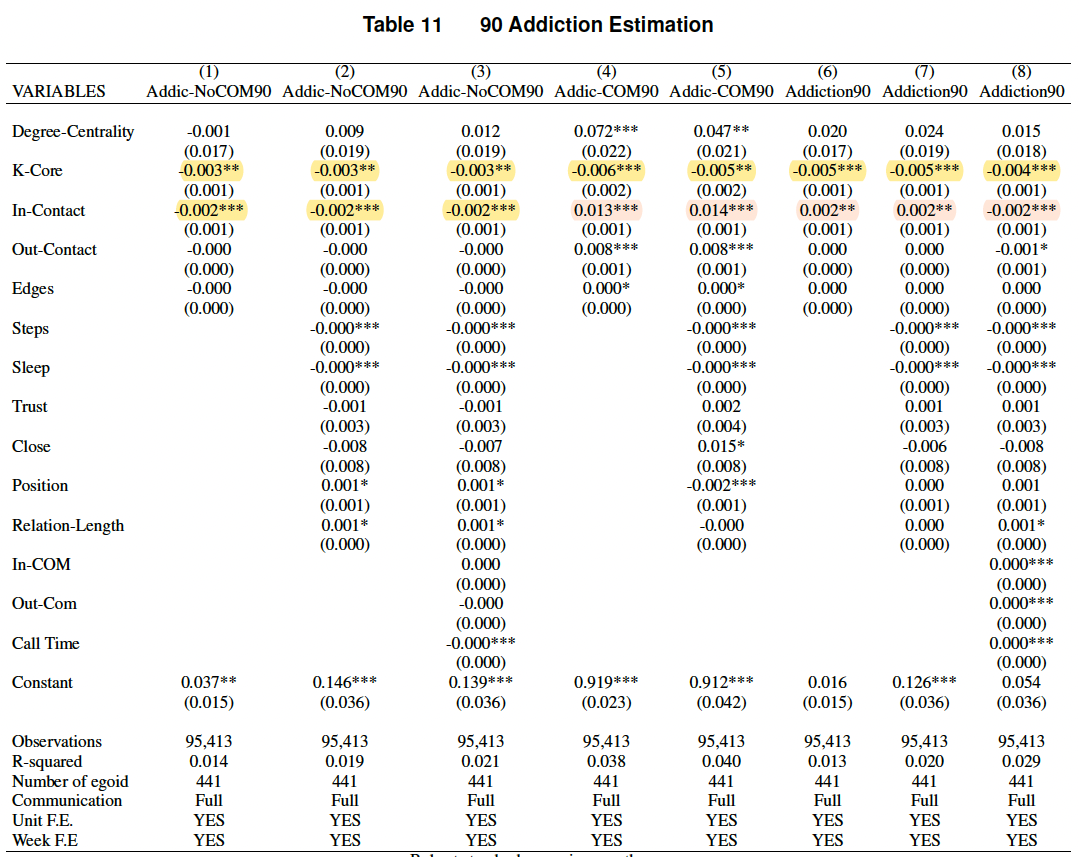
\includegraphics{images/addiction.png}

}

\end{figure}

\hypertarget{result-4-addiction-esimation-logistic-3}{%
\subsection{Result 4: Addiction Esimation
(Logistic)}\label{result-4-addiction-esimation-logistic-3}}

\begin{figure}

{\centering 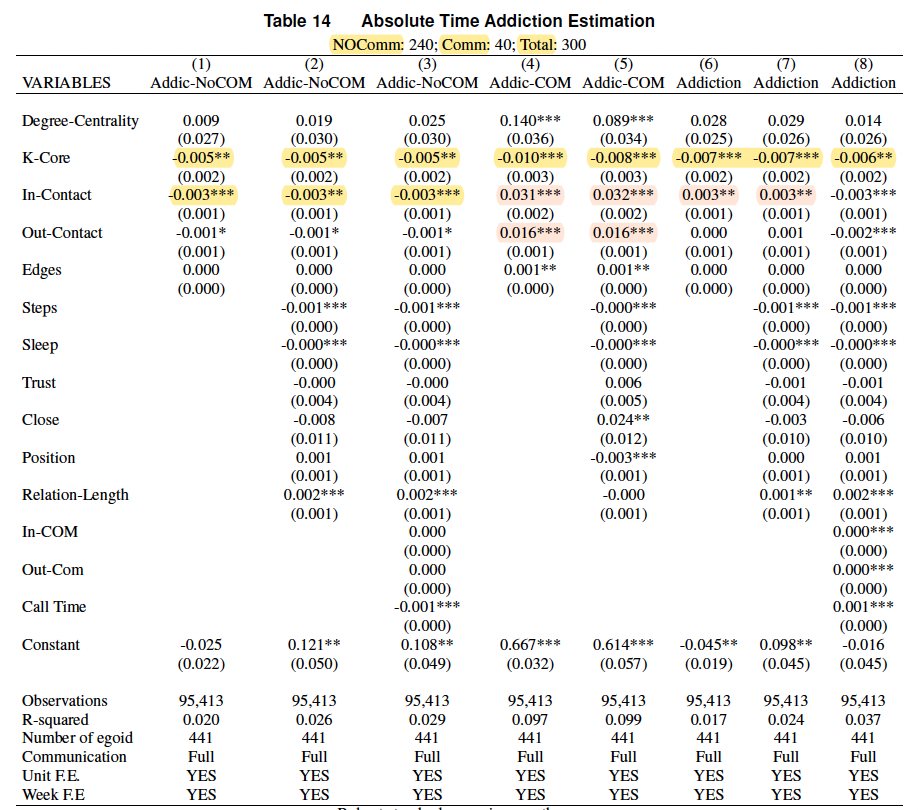
\includegraphics{images/addiction2-02.png}

}

\end{figure}

\hypertarget{conclusion-4-h4}{%
\subsection{Conclusion 4 (H4)}\label{conclusion-4-h4}}

~

\begin{itemize}
\tightlist
\item
  Network features \textbf{outperform} traditional constructs (Trust,
  Social Distance (Closeness)).
\end{itemize}

\hypertarget{result-4-sleep-as-dv}{%
\subsection{Result 4: Sleep as DV}\label{result-4-sleep-as-dv}}

\begin{itemize}
\tightlist
\item
  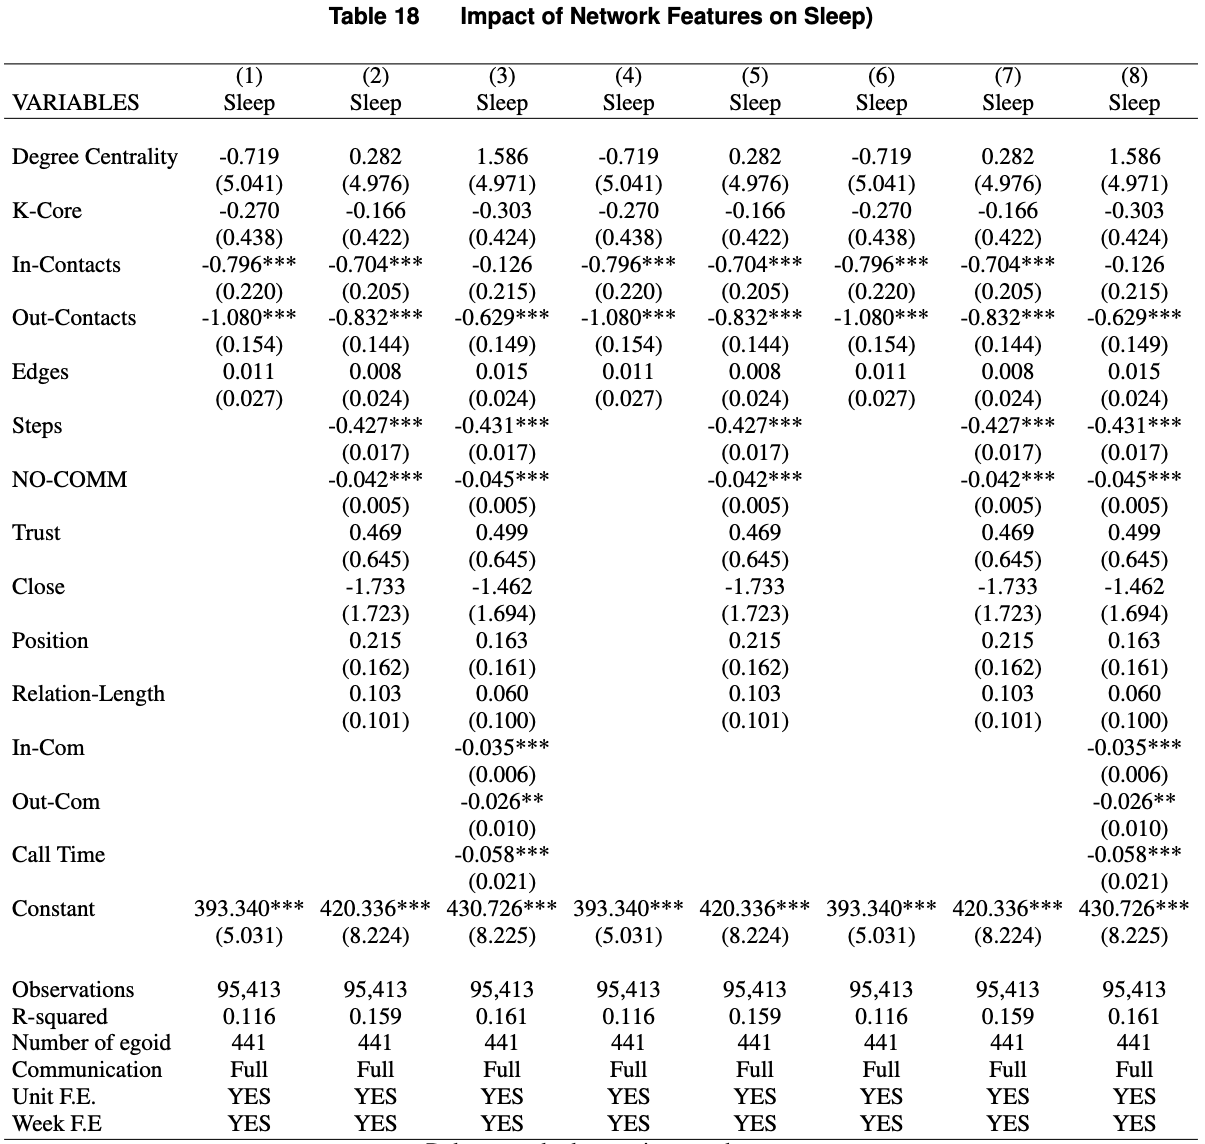
\includegraphics{images/2sleep.png}
\end{itemize}



\end{document}
